\documentclass[12pt]{report}
\usepackage{fontspec}
\usepackage{graphicx}
\usepackage{geometry}
\usepackage{fancyhdr}
\usepackage{changepage}
\usepackage{enumitem}
\usepackage[colorlinks=true, linkcolor=blue, urlcolor=blue, citecolor=blue]{hyperref}


\geometry{
  a4paper,
  top=1.5cm,
  bottom=2.0cm,
  left=2.0cm,
  right=2.0cm
}


% Khmer and English fonts
\newfontfamily\khmerfont{Khmer OS Muol Light}
\newfontfamily\khmernormal{Khmer OS Siemreap}
\newfontfamily\englishfont{TeX Gyre Termes}




\XeTeXlinebreaklocale "khmer"
\XeTeXlinebreakskip = 0pt plus 1pt

\title{}
\author{}
\date{}

\begin{document}

% Title page with no page number
\begin{titlepage}
    \centering
    \vspace*{1cm}

    \begin{minipage}{0.25\textwidth}
        
\includegraphics[width=3.5cm]{figures/RUPP.jpg}
    \end{minipage}
    \hfill
    \begin{minipage}{0.65\textwidth}
        \raggedright
        {\khmerfont\fontsize{16pt}{20pt}\selectfont សាកលវិទ្យាល័យភូមិន្ទភ្នំពេញ\\[0.6em]}
        {\large\bfseries ROYAL UNIVERSITY OF PHNOM PENH}
    \end{minipage}

    \vspace{2cm}

    \begin{minipage}{0.9\textwidth}
        \centering
        {\khmerfont\fontsize{12pt}{20pt}\selectfont ការស្រាវជ្រាវវិធីសាស្ដ្រថ្មី  សម្រាប់កំណត់សម្គាល់អត្ថបទអក្សរខ្មែរទូទៅ នឹងបានប្រើប្រាស់ស្ថាបត្យកម្ម {\englishfont\textbf{Craft}} ជាមួយនឹង {\englishfont\textbf{TrOCR}}\\[0.4em]}
        {\englishfont\fontsize{15pt}{20pt}\selectfont\bfseries A novel End-to-End approach for General Khmer Text \par}
        {\englishfont\fontsize{15pt}{20pt}\selectfont\bfseries Recognition using Craft with TrOCR Architecture \par}
    \end{minipage}

    \vspace{3.0cm}

    {\englishfont\fontsize{16pt}{20pt}\selectfont Mr. Vitou Soy\par}

    \vspace{3.0cm}

    {\englishfont\fontsize{16pt}{20pt}\selectfont A Thesis\par}
    \vspace{0.5cm}
    {\large In Partial Fulfilment of the Requirement for the Degree of\par}
    {\large Bachelor of Engineering in Information-Technology-Engineering\par}
    

    \vspace{2.5cm}

    {\englishfont
    \begin{center}
        \begin{tabular}{ll}
            {Examination committee:} & Mr. Sokchea Kor (Advisor) \\
                                    & Mr. Chanpiseth Chap (committee) \\
                                    & Mrs. Daly Chea (committee)\\
                                    & Dr. \dotfill
        \end{tabular}
    \end{center}
    }

    \vfill
    {\Large\bfseries June 2025\par}
\end{titlepage}

\thispagestyle{empty}


% --- Abstract Page (Khmer) ---
\thispagestyle{plain}
\begin{adjustwidth}{0.2cm}{0.2cm}

    % Khmer Abstract
    \begin{center}
        {\khmerfont\fontsize{15pt}{25pt}\selectfont សង្ខេបសេចក្ដី \par}
    \end{center}
    \phantomsection
    \label{khmer-abstract}
    \vspace{0.5cm}
    \khmernormal
    \small
    ក្នុងសហគមន៍បច្ចេកវិទ្យាព័ត៌មានសម័យថ្មី ការចាប់យកអត្ថបទចេញពីរូបភាព  – [ OCR ]
    (Optical Character Recognition) ក្លាយជាបច្ចេកវិទ្យាសំខាន់មួយដែលត្រូវបានប្រើប្រាស់
    យ៉ាងទូលំទូលាយ សម្រាប់បំលែងឯកសារសរសេរ ឬរូបភាពអក្សរឱ្យទៅជាអត្ថបទ អេឡិចត្រូនិច (digital text)។ 
    ការអភិវឌ្ឍ OCR សម្រាប់ភាសាខ្មែរ តែងតែប្រឈមនឹងបញ្ហាជាច្រើន ដោយសារកង្វះនៃប្រភពទិន្នន័យ 
    និងឯកសារសម្រាប់ train AI model។ ដើម្បីដោះស្រាយបញ្ហានេះ យើងបានបង្កើតទិន្នន័យសិប្បនិម្មិត 
    (Synthetic Dataset) ដោយប្រើវិធីសាស្ត្របច្ចេកទេសកម្រិតខ្ពស់។\par
    
    ក្នុងដំណើរការបង្កើតទិន្នន័យសិប្បនិម្មិត (Synthetic Dataset) រួមមាន៖
    \begin{itemize}
        \item វិធីសាស្ដ្រក្នុងការប្រមូលអត្ថបទចេញពីអ៊ីនធឺណិត មានដូចខាងក្រោម (Scrape data) ៖
        \begin{itemize}
            \item ដំណាក់កាលទីមួយ៖ យើងបានប្រមូលអត្ថបទចេញពី khsearch.com, Chuon-Nath-Dictionary, Alpha-Word, Google-Word, និងចុងក្រោយគឺ Huggingface.com ។
            \item ដំណាក់កាលទីពីរ៖ យើងបានសម្អាត ទិន្នន័យទាំងអស់នោះ ឆ្លងកាត់ដំណើរការ ដូចជា លុបចោលតួរអក្សរណាដែលមិនសូវមាន វត្តមាននៅលើ រូបភាព ញឹកញាប់ និងបានលុបចោល តួរអក្សរណាដែល Fonts renders អត់ចេញ។
            \item ដំណាក់កាលទីបី៖ ដំណាក់កាលមួយនេះ យើងបានធ្វើការ កាត់ប្រយោគទាំងអស់នោះ ជាពាក្យៗ ដោយប្រើប្រាស់ library ឈ្មោះ khmer-nltk
            \item ដំណាក់កាលទីបួន៖ ចុងក្រោយ ក៏បានរៀបចំជា ប្រយោគដែល មានប្រវែង Random ពី ១ អក្សរ រហូតដល់ ១១០ អក្សរ ។
        \end{itemize}
        \item បង្កើតរូបភាពដោយអនុវត្តតាមលក្ខខណ្ឌខាងក្រោម ៖ 
        \begin{itemize}
            \item ផ្ទៃខាងក្រោយចៃដន្យ (Apply Different backgrounds)
            \item បំពាក់ពុម្ពអក្សរផ្សេងៗគ្នា (Apply Different fonts)
            \item Noise: \texttt{gaussian\_noise}, \texttt{salt\_pepper\_noise}, \texttt{speckle\_noise}, \texttt{blur}
            \item បង្វិលអក្សរបន្តិច (random rotation text)
            \item បញ្ចូល Margin Randomly (1, 5) pixels
        \end{itemize}
        \item សរុបមកយើងបានបង្កើត Data ជាង ៤ លាន records សម្រាប់ train OCR model
    \end{itemize}
    \par
    
    Architecture OCR ត្រូវបានបែងចែកជា ២ ផ្នែក៖ \textbf{Text Detection} និង \textbf{Text Recognition}:\par
    
    \textbf{Text Detection}: យើងប្រើម៉ូដែល \textbf{CRAFT} ដោយបានធ្វើការ Train ឡើងវិញដោយ បាន annotation ទៅលើ 
    លើរូបភាពប្រហែល ៥០០ images និងសរុបចំនួន bounding box ជាង ១០,០០០ boxes។\par
    
    \textbf{Text Recognition}: យើងប្រើ \textbf{TrOCR base model} ចេញពី Microsoft (មាននៅក្នុង Hugging Face) ហើយបាន
    fine-tune ទៅលើ dataset ខ្មែរសិប្បនិម្មិត (Synthetic Dataset) ដើម្បីបង្កើនសមត្ថភាពក្នុងការសម្គាល់អក្សរខ្មែរ។\par
    
    លទ្ធផលសិក្សាបានបង្ហាញថា OCR របស់ពួកយើងអាចសម្គាល់អត្ថបទចេញពីរូបភាព បានដោយភាពត្រឹមត្រូវលើសពី ៩០\%។ 
    ដូច្នេះ ការសិក្សានេះបង្ហាញអំពីសក្តានុពលនៃការបង្កើត dataset និងការប្រើម៉ូដែលជំនាន់ថ្មី ដើម្បីអភិវឌ្ឍន៍ OCR ភាសាខ្មែរឱ្យមានប្រសិទ្ធភាពកាន់តែខ្ពស់។
    វាមានសមត្ថភាព អាចចាប់យកអត្ថបទមិនត្រឹមតែពាក្យខ្លីៗ ប៉ុណ្ណោះទេ តែវាក៏អាចធ្វើការចាប់យក ដូចជា មួយតួអក្សរដោយមួយតួអក្សរ, ពាក្យដោយពាក្យ, ប្រយោគដោយប្រយោគ រហូតដល់ មួយប្រយោគវែង ១១០ តួអក្សរថែមទៀតផង ។ ហើយលើសពីនោះទៀត វាក៏អាចធ្វើការ កំណត់សម្គាល់ទៅលើ ពីរ ភាសាចម្បង ទាំងភាសាខ្មែរ និងភាសាអង់គ្លេស ។    
    \vspace{2cm}
    
    % English Abstract
    \begin{center}
        {\bfseries\LARGE Abstract \par}
    \end{center}
    \phantomsection
    \label{abstract}
    \vspace{0.5cm}
    \englishfont
    \large
    
    OCR technology continues to evolve rapidly, but Khmer text 
    recognition still presents challenges—mainly because of the 
    limited availability of high-quality training data. In this work, 
    we introduce an end-to-end OCR approach for both Khmer and English text, 
    tailored to work well even under low-resource conditions. Our pipeline combines 
    reliable text detection and advanced recognition techniques, designed to reflect real-world multilingual usage in Cambodia.

    We began by manually collecting a dataset of 1,000 real-world images, 
    carefully annotating 13,200 text-line bounding boxes in both Khmer and English. 
    This gave us a strong foundation to train our text detection model using CRAFT, 
    which excels at detecting irregular text regions. Training on our custom-annotated 
    data, the CRAFT model achieved strong performance, with 90\% recall, 89\% precision, 
    and an F1-score of 86.8\%. These results show that with focused annotation efforts, 
    high-quality detection is achievable even without large public datasets.
    
    To further improve the system’s performance and handle a wider variety of input, 
    we generated a synthetic training dataset using a text-to-image method. We 
    collected a large corpus of Khmer and English sentences from the web and used 
    this to create thousands of synthetic images simulating different fonts, layouts, 
    and noise patterns. This synthetic data expanded the diversity of our training 
    set and allowed the model to better generalize to unseen real-world samples.
    
    For the recognition stage, we used TrOCR—a transformer-based architecture built 
    for OCR tasks. However, the original TrOCR processor was not designed to support 
    Khmer text and could not correctly interpret the language. To address this, 
    we customized the processor so that it could properly tokenize and decode Khmer 
    characters. This modification was essential to ensure that the model could 
    understand and accurately transcribe Khmer script.
    
    After training on both real and synthetic data, our TrOCR-based recognition model 
    showed strong results on real-world test images: a character error rate (CER) 
    of 0.02 overall, with 0.04 for Khmer, 0.01 for English, and 0.06 for lines 
    containing both languages.
    
    One of the key motivations behind this work is the increasing use of English 
    in Cambodia. While Khmer remains the national language, English is now widely 
    used as a second language and often appears alongside Khmer in signs, documents, 
    and digital platforms. By building a system that supports both languages, 
    we aim to match the multilingual nature of everyday text in Cambodia.
    
    Finally, unlike most academic research that never reaches real-world usage, 
    we’ve made our OCR system publicly accessible through a production-ready API. 
    This allows others to test and integrate the model into their own applications, 
    bridging the gap between research and practical deployment. According to recent 
    studies, nearly 80\% of research models never get deployed or made accessible—our 
    goal was to break that trend. By turning our model into a usable, open API, 
    we ensure that the results of this work are not only measurable in papers 
    but also usable by the community.


    
    \end{adjustwidth}
\newpage

% --- Supervisor Statement Page (Khmer) ---
\thispagestyle{plain}
\begin{adjustwidth}{0.2cm}{0.2cm}


    % supervisor statement
    \begin{center}
        {\englishfont\fontsize{14pt}{21pt}\selectfont \textbf{SUPERVISOR's RESEARCH SUPERVISION STATEMENT} \par}
    \end{center}
    \phantomsection
    \label{supervisor-statement}

    \vspace{1cm}
    
    \englishfont\large
    \begin{flushleft}
    Name of program: Khmer Studies\par
    Name of candidate: Vitou Soy\par
    \end{flushleft}

    \vspace{1cm}
    
    \englishfont\large
    \begin{flushleft}
    Title of research report: A novel End-to-End approach for General Khmer Text
    Recognition using Craft with TrOCR Architecture\par
    \end{flushleft}

    \vspace{1cm}
    \setlength{\parindent}{0pt}
    This is to certify that the research carried out for the above titled master's
    research report was completed by the above named candidate under my direct
    supervision. This thesis material has not been used for any other degree. The
    candidate has demonstrated strong research capabilities and independence in
    developing novel approaches for Khmer text recognition. The research
    methodology, implementation, and results are original contributions to the field
    of Khmer OCR technology. I have provided guidance and oversight throughout
    the research process while allowing the candidate to explore innovative
    solutions.\par

    \vspace{1cm}
    \begin{flushleft}
    Supervisor's name: Sokchea Kor\par
    \vspace{0.1cm}
    Supervisor's signature:……………………\par
    \vspace{0.1cm}
    Date……………………………………………\par
    \end{flushleft}

\end{adjustwidth}
\newpage

% --- Candidate Statement Page (Khmer) ---
\thispagestyle{plain}
\begin{adjustwidth}{0.2cm}{0.2cm}

% supervisor statement
\begin{center}
    {\englishfont\fontsize{14pt}{21pt}\selectfont \textbf{CANDIDATE'S STATEMENT} \par}
\end{center}
\label{candidate-statement}

\vspace{1cm}
{\englishfont\fontsize{12pt}{18pt}\selectfont \setlength{\parindent}{0pt} TO WHOM IT MAY CONCERN \par}

\vspace{0.5cm}
    \setlength{\parindent}{0pt}
    {\large This is to certify that the dissertation that I, Vitou Soy, hereby present, entitled "Advancing
    Khmer Optical Character Recognition: A Synthetic Data-Driven Approach," for the degree
    of Bachelor of Engineering in Information Technology at the Royal University of Phnom Penh, is
    entirely my own work. Furthermore, it has not been used to fulfill the requirements of any
    other qualification, in the whole or in part, at this or any other University or equivalent
    institution. The research methodology, implementation, and findings represent original con-
    tributions to the field of Khmer OCR technology, particularly in developing novel approaches
    for synthetic data generation and transformer-based text recognition. Through this work, I
    have demonstrated strong research capabilities and independence in addressing the critical
    challenges of Khmer text digitization and recognition.\par}

    \vspace{0.5cm}
    \setlength{\parindent}{0pt}
    {\large No reference to, or quotation from, this document may be made without the written
    approval of the author.\par}
    \vspace{1cm}
    \setlength{\parindent}{0pt}
    {\large Name of Candidate: Vitou Soy\par}
    
    \vspace{0.5cm}
    \setlength{\parindent}{0pt}
    {\large Signed by the candidate: \hspace{1cm}\raisebox{-1ex}{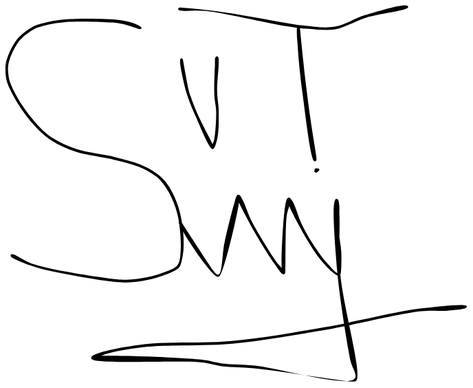
\includegraphics[width=1cm]{figures/sign_cadidate.png}}\hspace{\fill}\par}
    
    \vspace{0.5cm}
    \setlength{\parindent}{0pt}
    {\large Date: \dotfill\par}

    \vspace{1cm}
    \setlength{\parindent}{0pt}
    {\large Name of Supervisor: Mr. Sokchea Kor\par}
    
    \vspace{0.5cm}
    \setlength{\parindent}{0pt}
    {\large Countersigned by the Supervisor: \dotfill\par}
    
    \vspace{0.5cm}
    \setlength{\parindent}{0pt}
    {\large Date: \dotfill\par}

    
\end{adjustwidth}
\newpage

% --- Acknowledgments Page (Khmer) ---
\thispagestyle{plain}
\begin{adjustwidth}{0.2cm}{0.2cm}

    % Acknowledgments
    \begin{center}
        {\englishfont\fontsize{14pt}{21pt}\selectfont \textbf{ACKNOWLEDGMENTS} \par}
    \end{center}
    \phantomsection
    \label{acknowledgements}

    \vspace{1cm}
    \setlength{\parindent}{2em}
    {\large I would like to begin by expressing my sincere gratitude for the opportunity to pursue this research. I am deeply thankful to the Royal University of Phnom Penh for offering such a well-structured academic program within the Faculty of Engineering, which has provided a strong foundation for this success. The comprehensive curriculum, practical exposure, and academic environment have been instrumental in shaping my journey.

    \vspace{0.5cm}
    I am especially grateful to all the faculty members for their dedicated teaching and continuous support throughout my studies. Their commitment to student learning has inspired and guided me significantly. I would also like to thank my classmates for their collaboration, encouragement, and the shared experiences that made this journey memorable.

    \vspace{0.5cm}
    My deepest appreciation goes to my supervisor, Mr. Kor Sokchea, whose expertise, mentorship, and unwavering support have been vital to the completion of this work. He has been not only an exceptional lecturer and supervisor but also a strong supporter at every stage. This research would not have been possible without his guidance.

    \vspace{0.5cm}
    Finally, I want to express my heartfelt thanks to my family for their financial support, constant encouragement, and unconditional love. Their sacrifices and belief in me have been the driving force behind my achievements. I am especially grateful to my sister, who has always believed in me and supported every decision I made—thank you for always standing by my side.

    \par}

\end{adjustwidth}

\newpage

% --- Table of Contents Page (Khmer) ---
\thispagestyle{plain}
\begin{adjustwidth}{0.2cm}{0.2cm}

    \begin{center}
        {\englishfont\fontsize{14pt}{21pt}\selectfont \textbf{TABLE OF CONTENTS} \par}
    \end{center}
    \phantomsection
    \label{toc}

    \vspace{1cm}

    \setlength{\parindent}{0pt}
    {\large \textbf{Preliminary Pages}\par}
    \vspace{0.3cm}
    {\khmernormal\fontsize{11pt}{16pt}\selectfont មូលន័យសង្ខេប\dotfill\hyperref[khmer-abstract]{{\pageref{khmer-abstract}}}\hspace{0.1cm}\par}
    {\large Abstract\dotfill\hyperref[abstract]{{\pageref{abstract}}}\hspace{0.1cm}\par}
    {\large Supervisor's Research Supervision Statement\dotfill\hyperref[supervisor-statement]{{\pageref{supervisor-statement}}}\hspace{0.1cm}\par}
    {\large Candidate's Statement\dotfill\hyperref[candidate-statement]{{\pageref{candidate-statement}}}\hspace{0.1cm}\par}
    {\large Acknowledgements\dotfill\hyperref[acknowledgements]{{\pageref{acknowledgements}}}\hspace{0.1cm}\par}
    {\large Table of Contents\dotfill\hyperref[toc]{{\pageref{toc}}}\hspace{0.1cm}\par}
    {\large List of Tables\dotfill\hyperref[lot]{{\pageref{lot}}}\hspace{0.1cm}\par}
    {\large List of Figures\dotfill\hyperref[lof]{{\pageref{lof}}}\hspace{0.1cm}\par}
    {\large List of Abbreviations\dotfill\hyperref[loa]{{\pageref{loa}}}\hspace{0.1cm}\par}

    \vspace{0.5cm}
    {\large \textbf{Chapter 1: Introduction}\dotfill\pageref{ch:intro}\par}
    {\large 1.1 Background to the Study\dotfill\pageref{sec:background}\par}
    {\large 1.2 Problem Statement\dotfill\pageref{sec:problem}\par}
    {\large 1.3 Aim and Objectives of the Study\dotfill\pageref{sec:objectives}\par}
    {\large 1.4 Research Questions\dotfill\pageref{sec:questions}\par}
    {\large 1.5 Rationale of the Study\dotfill\pageref{sec:rationale}\par}
    {\large 1.6 Limitations and Scope\dotfill\pageref{sec:limitations}\par}
    {\large 1.7 Structure of the Thesis\dotfill\pageref{sec:structure}\par}

    \vspace{0.5cm}
    {\large \textbf{Chapter 2: Literature Review}\dotfill\pageref{ch:literature}\par}
    {\large 2.1 Overview\dotfill\pageref{sec:ocr-overview}\par}
    {\large 2.2 Definition of Optical Character Recognition (OCR)\dotfill\pageref{sec:ocr-definition}\par}

    \vspace{0.5cm}
    {\large \textbf{Chapter 3: Dataset Construction}\dotfill\pageref{ch:dataset}\par}
    {\large 3.1 Text Source Collection\dotfill\pageref{sec:text-source}\par}
    {\large \hspace{1cm}3.1.1 Khmer Websites and Dictionaries\dotfill\pageref{subsec:websites}\par}
    {\large \hspace{1cm}3.1.2 Online NLP Resources and Tools\dotfill\pageref{subsec:nlp-tools}\par}
    {\large 3.2 Text Cleaning and Preprocessing\dotfill\pageref{sec:preprocessing}\par}
    {\large \hspace{1cm}3.2.1 Removal of Invalid Characters and Whitespace\dotfill\pageref{subsec:cleaning}\par}
    {\large \hspace{1cm}3.2.2 Unicode Normalization\dotfill\pageref{subsec:unicode}\par}
    {\large 3.3 Sentence Segmentation and Reconstruction\dotfill\pageref{sec:segmentation}\par}
    {\large \hspace{1cm}3.3.1 Tokenization Using khmer-nltk\dotfill\pageref{subsec:tokenization}\par}
    {\large \hspace{1cm}3.3.2 Sentence Length Variation\dotfill\pageref{subsec:length}\par}
    {\large 3.4 Image Generation Pipeline\dotfill\pageref{sec:generation}\par}
    {\large \hspace{1cm}3.4.1 Font and Background Selection\dotfill\pageref{subsec:fonts}\par}
    {\large \hspace{1cm}3.4.2 Noise Injection Techniques\dotfill\pageref{subsec:noise}\par}
    {\large \hspace{1cm}3.4.3 Image Rotation and Margin Augmentation\dotfill\pageref{subsec:augmentation}\par}
    {\large 3.5 Dataset Statistics and Format\dotfill\pageref{sec:statistics}\par}
    {\large 3.6 Comparison with Existing Datasets\dotfill\pageref{sec:comparison}\par}

    \vspace{0.5cm}
    {\large \textbf{Chapter 4: Experiments}\dotfill\pageref{ch:experiments}\par}
    {\large 4.1 Experimental Environment and Tools\dotfill\pageref{sec:environment}\par}
    {\large 4.2 Model Architecture and Configuration\dotfill\pageref{sec:architecture}\par}
    {\large \hspace{1cm}4.2.1 CRAFT for Text Detection\dotfill\pageref{subsec:craft}\par}
    {\large \hspace{1cm}4.2.2 TrOCR for Text Recognition\dotfill\pageref{subsec:trocr}\par}
    {\large 4.3 Training Methodology\dotfill\pageref{sec:training}\par}
    {\large \hspace{1cm}4.3.1 Fine-tuning CRAFT on Annotated Images\dotfill\pageref{subsec:craft-training}\par}
    {\large \hspace{1cm}4.3.2 Fine-tuning TrOCR on Synthetic Dataset\dotfill\pageref{subsec:trocr-training}\par}
    {\large 4.4 Evaluation Metrics\dotfill\pageref{sec:metrics}\par}
    {\large \hspace{1cm}4.4.1 Detection Metrics (Precision, Recall)\dotfill\pageref{subsec:detection-metrics}\par}
    {\large \hspace{1cm}4.4.2 Recognition Metrics (Accuracy, CER, WER)\dotfill\pageref{subsec:recognition-metrics}\par}
    {\large 4.5 Baseline and Benchmark Comparison\dotfill\pageref{sec:benchmark}\par}

    \vspace{0.5cm}
    {\large \textbf{Chapter 5: Results and Analysis}\dotfill\pageref{ch:results}\par}
    {\large 5.1 Text Detection Results\dotfill\pageref{sec:detection-results}\par}
    {\large \hspace{1cm}5.1.1 Quantitative Metrics\dotfill\pageref{subsec:quantitative}\par}
    {\large \hspace{1cm}5.1.2 Qualitative Visual Examples\dotfill\pageref{subsec:qualitative}\par}
    {\large 5.2 Text Recognition Results\dotfill\pageref{sec:recognition-results}\par}
    {\large \hspace{1cm}5.2.1 Accuracy on Character, Word, Sentence Levels\dotfill\pageref{subsec:accuracy}\par}
    {\large \hspace{1cm}5.2.2 Performance Across Sentence Lengths\dotfill\pageref{subsec:performance}\par}
    {\large 5.3 Khmer vs. English Performance\dotfill\pageref{sec:comparison-results}\par}
    {\large 5.4 Error Analysis and Failure Cases\dotfill\pageref{sec:error-analysis}\par}
    {\large 5.5 System Robustness and Generalization\dotfill\pageref{sec:robustness}\par}

    \vspace{0.5cm}
    {\large \textbf{Chapter 6: Discussion}\dotfill\pageref{ch:discussion}\par}
    {\large 6.1 Effectiveness of Synthetic Data\dotfill\pageref{sec:effectiveness}\par}
    {\large 6.2 Strengths and Limitations of the OCR System\dotfill\pageref{sec:strengths}\par}
    {\large 6.3 Research Challenges and Lessons Learned\dotfill\pageref{sec:challenges}\par}
    {\large 6.4 Comparison with Related Works\dotfill\pageref{sec:related-works}\par}
    {\large 6.5 Impact on Khmer NLP and OCR Research\dotfill\pageref{sec:impact}\par}

    \vspace{0.5cm}
    {\large \textbf{Chapter 7: Conclusion and Future Work}\dotfill\pageref{ch:conclusion}\par}
    {\large 7.1 Summary of Contributions\dotfill\pageref{sec:contributions}\par}
    {\large 7.2 Key Findings\dotfill\pageref{sec:findings}\par}
    {\large 7.3 Limitations\dotfill\pageref{sec:final-limitations}\par}
    {\large 7.4 Future Research Directions\dotfill\pageref{sec:future}\par}
    {\large 7.5 Final Remarks\dotfill\pageref{sec:remarks}\par}

    \vspace{0.5cm}
    {\large \textbf{Chapter 8: Practical Applications}\dotfill\pageref{ch:applications}\par}
    {\large 8.1 Use in Document Digitization\dotfill\pageref{sec:digitization}\par}
    {\large 8.2 OCR for Education and Cultural Preservation\dotfill\pageref{sec:preservation}\par}
    {\large 8.3 Deployment Considerations\dotfill\pageref{sec:deployment}\par}
    {\large 8.4 Opportunities for Government and Enterprise Use\dotfill\pageref{sec:opportunities}\par}

    \vspace{0.5cm}
    {\large \textbf{References}\dotfill\pageref{ch:references}\par}

    \vspace{0.5cm}
    {\large \textbf{Appendices}\par}
    {\large Appendix A: Sample Annotated Images\dotfill\pageref{appendix-a}\par}
    {\large Appendix B: List of Fonts Used\dotfill\pageref{appendix-b}\par}
    {\large Appendix C: Code Snippets and Training Configuration\dotfill\pageref{appendix-c}\par}
    {\large Appendix D: Additional Evaluation Examples\dotfill\pageref{appendix-d}\par}

\end{adjustwidth}

\newpage

% --- List of Tables Page (Khmer) ---
\thispagestyle{plain}
\begin{adjustwidth}{0.2cm}{0.2cm}

    \begin{center}
        {\englishfont\fontsize{14pt}{21pt}\selectfont \textbf{List of Tables} \par}
    \end{center}
    \phantomsection
    \label{lot}

    \vspace{1cm}
    \setlength{\parindent}{0pt}
    \vspace{0.3cm}
    {\large Table 1.1: Compare Model\dotfill\pageref{abstract}\hspace{0.1cm}\par}

\end{adjustwidth}
\newpage

% --- List of Figures Page (Khmer) ---
\thispagestyle{plain}
\begin{adjustwidth}{0.2cm}{0.2cm}

    \begin{center}
        {\englishfont\fontsize{14pt}{21pt}\selectfont \textbf{List of Figures} \par}
    \end{center}
    \label{lof}

    \vspace{1cm}
    \setlength{\parindent}{0pt}
    \vspace{0.3cm}
    {\large Figure 1.1: Experiment Result\dotfill\pageref{abstract}\hspace{0.1cm}\par}

\end{adjustwidth}
\newpage

% --- List of Abbreviations Page (Khmer) ---
\thispagestyle{plain}
\begin{center}
    {\englishfont\fontsize{14pt}{21pt}\selectfont \textbf{LIST OF ABBREVIATIONS} \par}
\end{center}
\phantomsection
\label{loa}
\addcontentsline{toc}{chapter}{List of Abbreviations}

\begin{adjustwidth}{0.2cm}{0.2cm}

    \vspace{1cm}
    \setlength{\parindent}{0pt}
    \vspace{0.3cm}
    {\large AI: Artificial Intelligence\dotfill\par}
    {\large API: Application Programming Interface\dotfill\par}
    {\large BART: Bidirectional and Auto-Regressive Transformers\dotfill\par}
    {\large CER: Character Error Rate\dotfill\par}
    {\large CNN: Convolutional Neural Network\dotfill\par}
    {\large CRAFT: Character Region Awareness for Text Detection\dotfill\par}
    {\large CTC: Connectionist Temporal Classification\dotfill\par}
    {\large DCT: Discrete Cosine Transform\dotfill\par}
    {\large EAST: Efficient and Accurate Scene Text Detector\dotfill\par}
    {\large GPU: Graphics Processing Unit\dotfill\par}
    {\large Grad-CAM: Gradient-weighted Class Activation Mapping\dotfill\par}
    {\large HMM: Hidden Markov Model\dotfill\par}
    {\large HTK: Hidden Markov Model Toolkit\dotfill\par}
    {\large ICDAR: International Conference on Document Analysis and Recognition\dotfill\par}
    {\large IoU: Intersection over Union\dotfill\par}
    {\large LSTM: Long Short-Term Memory\dotfill\par}
    {\large MLP: Multilayer Perceptron\dotfill\par}
    {\large NAR: Non-Autoregressive\dotfill\par}
    {\large NLP: Natural Language Processing\dotfill\par}
    {\large OCR: Optical Character Recognition\dotfill\par}
    {\large RAM: Random Access Memory\dotfill\par}
    {\large RNN: Recurrent Neural Network\dotfill\par}
    {\large Seq2Seq: Sequence-to-Sequence\dotfill\par}
    {\large SOM: Self-Organizing Map\dotfill\par}
    {\large SVM: Support Vector Machine\dotfill\par}
    {\large TrOCR: Transformer Optical Character Recognition\dotfill\par}
    {\large URL: Uniform Resource Locator\dotfill\par}
    {\large VGG: Visual Geometry Group\dotfill\par}
    {\large ViT: Vision Transformer\dotfill\par}
    {\large VRAM: Video Random Access Memory\dotfill\par}
    {\large WER: Word Error Rate\dotfill\par}
    {\large YOLO: You Only Look Once\dotfill\par}

\end{adjustwidth}
\newpage


% Enable normal page numbering (centered at bottom)
\pagestyle{plain}

\clearpage
\pagenumbering{arabic}
\setcounter{page}{1}

\phantomsection
\label{ch:intro}
\chapter{Introduction}

% This chapter presents about what is OCR? why it is needed, and
% what are the challenges in OCR. It also presents the problem 
% for OCR on Khmer script (non-latin based), and OCR on multilingual
% language such as Khmer and English. We will talk about the scope
% of this research because it'll help us to keep 
% our research scope ensures clarity, direction, and feasibility 
% throughout the study.

\section{Background to the Study}
\label{sec:background}

Optical Character Recognition (OCR) has changed how we 
turn printed text into digital formats. Thanks to AI 
advances, OCR systems now use deep learning to detect 
and classify characters from images. This technology 
powers digital libraries, search systems, and language 
processing tools.
OCR works great for major languages like English, 
Chinese, and Japanese. These languages have tons 
of training data and well-studied text structures. 
However, OCR for complex-script languages like Khmer
is still limited.
Cambodia needs OCR technology more than ever. 
Over the past 20 years, the country has gone digital 
fast. People want to digitize Khmer documents for 
education, research, and everyday use, but here's 
the problem: Khmer script is incredibly complex.
Khmer writing goes back to the 7th century. It's 
not like English where letters sit in a row. Khmer 
characters stack on top of each other. They have 
subscripts, diacritics, and vowel markers that can 
appear above, below, or around the main character. 
Miss one tiny mark and you change the whole meaning 
of a word.

\begin{table}[H]
    \caption{Why Khmer OCR is Desperately Needed}
    \vspace{10pt}
    \phantomsection
    \label{sec:textbook}
    \resizebox{\textwidth}{!}{
    \begin{tabular}{|l|l|l|}
    \hline
    Sector & Current Problem & Impact \\
    \hline
    Education & Physical textbooks only & Students can't search or edit content \\
    Libraries & Books rotting on shelves & Knowledge becomes inaccessible \\
    Government & Paper records everywhere & Slow bureaucracy, hard to find documents \\
    Healthcare & Handwritten patient files & Doctors waste time, medical errors increase \\
    Business & Manual data entry & Companies lose money on inefficiency \\
    Culture & Ancient texts deteriorating & We're losing our heritage \\
    \hline
    \end{tabular}
    }
\end{table}

Look at education. Most school textbooks exist only on paper. The original digital files? Gone. Lost. This creates real problems for students who need accessible learning materials.

But it's bigger than just schools. Ancient palm leaf manuscripts are crumbling. Government documents pile up in storage rooms. Hospitals still use paper files that doctors can't read properly. Businesses waste hours typing data that OCR could handle in minutes.

And here's what's really frustrating: while Google can read English text perfectly, it struggles with basic Khmer sentences. The technology gap is huge.

The thing is, Khmer OCR isn't just a nice to have anymore. It's essential for Cambodia's digital future. The country needs this technology to preserve its culture, modernize its institutions, and give its people better access to information.

That's exactly why this research matters. We're not just building another OCR system. We're creating technology that could unlock thousands of years of Khmer knowledge and make it searchable, editable, and accessible to everyone.


\section{Problem Statement}
\label{sec:problem}

To develop OCR for English is really hard, but the way much more harder than you think is 
OCR on mixing languages such as English and Khmer. Most OCR systems work great with English because English is simple. Letters sit 
in a line. You read left to right, and Done.

For Khmer, that's a completely different beast. Characters stack on top of each other. 
They have tiny marks above and below that change the meaning. Miss one little dot 
and you've got the wrong word entirely.

\begin{figure}[H]
    \centering
    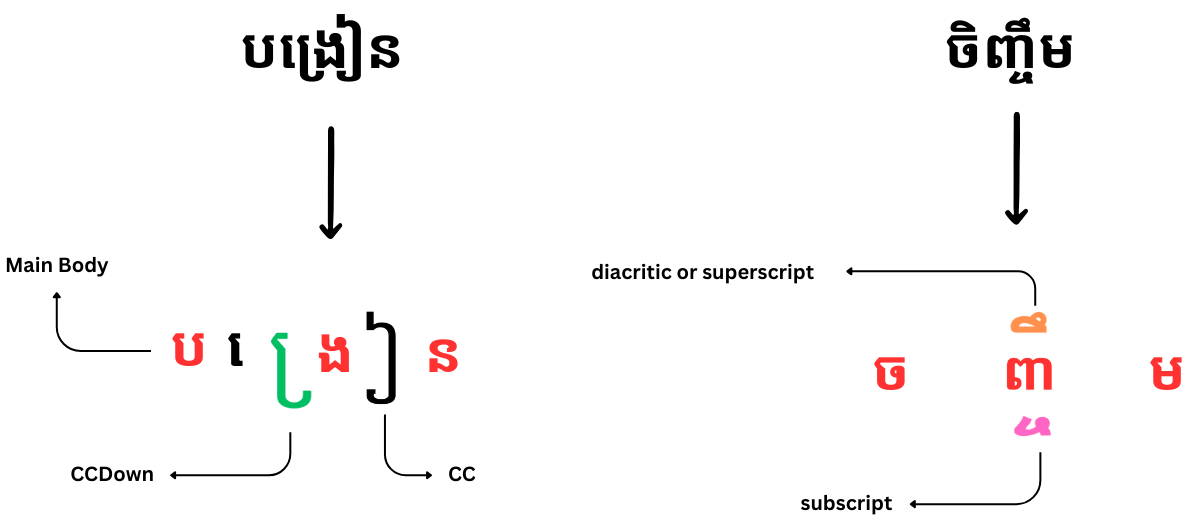
\includegraphics[width=\textwidth]{figures/example_of_text_format.png}
    \caption{Example of Khmer text format showing the complexity of character combinations and diacritics}
    \label{fig:text_format}
\end{figure}

Here's what makes Khmer OCR so different. First, there are no clear word breaks. 
In English, they use spaces between words (it's easy for AI to detect word level). 
Khmer writers use spaces sometimes, sometimes they don't, as you can see in figure
\ref{fig:sequential_text}, so it's really inconsistencies wirting system. This 
makes it impossible to know where one word ends and another begins.

\begin{figure}[H]
    \centering
    
\includegraphics[width=\textwidth]{figures/example_of_long_text.png}
    \caption{Example of sequential Khmer text showing how characters combine to form syllables and words}
    \label{fig:sequential_text}
\end{figure}

A growing challenge in modern Cambodia is the increasing prevalence of mixed-language 
documents that combine Khmer and English text. As English education and international 
business have expanded over the past two decades, it's become common to see documents, 
signs, textbooks, and digital content that seamlessly blend both languages within the 
same sentence or paragraph.

\begin{figure}[H]
    \centering
    
\includegraphics[width=\textwidth]{figures/mix_language_khmer_and_english.png}
    \caption{Example of mixed Khmer-English text showing how both languages appear together in modern Cambodian documents}
    \label{fig:mix_language}
\end{figure}

This mixed-language phenomenon creates several specific problems for OCR systems:
\begin{itemize}
    \item \textbf{Script switching confusion:} OCR models must quickly adapt between completely different writing systems within the same text line
    \item \textbf{Different text layouts:} English flows horizontally while Khmer has vertical stacking, creating complex spatial relationships
    \item \textbf{Font inconsistencies:} The same document often uses different fonts for Khmer and English portions, confusing recognition model
\end{itemize}

Most existing Khmer OCR systems are designed for single-language scenarios 
and perform poorly when encountering this mixed-language reality 
that's everywhere in Cambodia today. Then there's the data problem. To develop high 
accuracy OCR model needs tons of millions annotated images. English has millions 
of labeled images already, How about Khmer lanugage? 
Finding sufficient training data presents a significant challenge. 
While English has millions of labeled training samples, Khmer language 
resources are extremely limited, with only a few thousand quality annotated 
samples available. The situation becomes even more challenging when seeking 
properly labeled mixed-language datasets that combine Khmer and English text. Without enough 
training data, OCR model stays dumb. It can't learn the 
patterns to recognize text accurately.

\begin{figure}[H]
    \centering
    
\includegraphics[width=\textwidth]{figures/varianty_of_font.png}
    \caption{Examples of the same Khmer text rendered in different fonts, demonstrating the significant visual variations that OCR systems must handle}
    \label{fig:font_variants}
\end{figure}

And let's talk about fonts. English has maybe around 15 to 25 common fonts that most people use,
based on reported study use case, from website such as rigorousthemes.com, lifehack.org, and indeed.com. 
Khmer has many different fonts that look very unique from each other, some are thick and bold, others are 
thin and delicate, some have fancy decorations. To train model on one font and 
it fails completely on another.

Look at Figure \ref{fig:font_variants}. Same text, different fonts. To a human, 
it's obviously the same sentence, to a computer, it might be different look.

\begin{figure}[H]
    \centering
    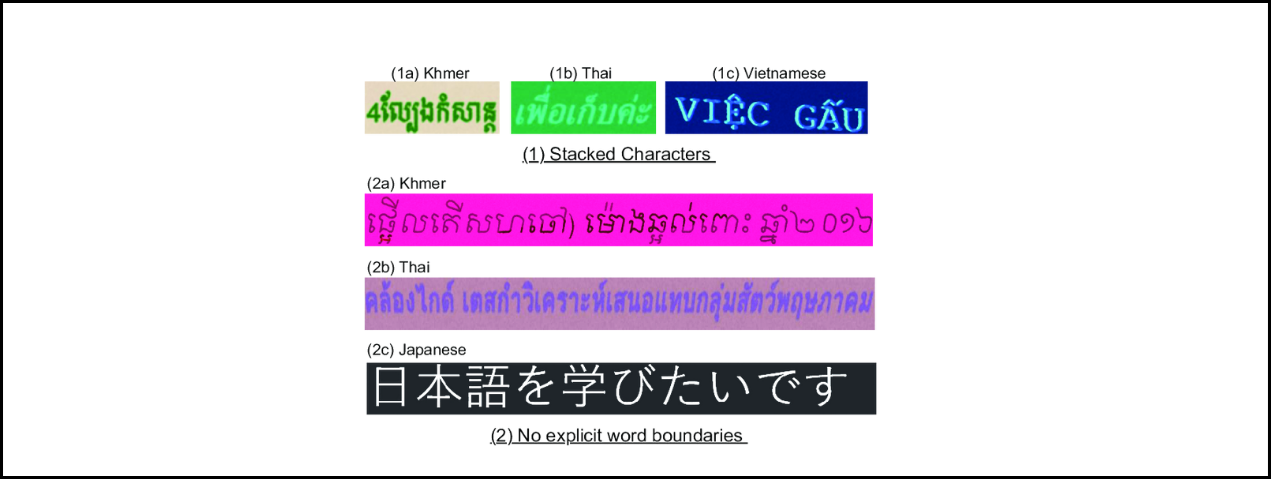
\includegraphics[width=\textwidth]{figures/text_stacking_mixing_language.png}
    \caption{Illustration of Khmer text stacking patterns, 
    showing how characters combine vertically and horizontally 
    to form syllables and words \citep{buoy2023khmerocr}}
    \label{fig:text_stacking}
\end{figure}

That's exactly why we need a better approach. Current OCR tools aren't 
built for the messy reality of Khmer text. They expect perfect conditions
and worked with char-level, word-level only,
that just don't exist in the real world.

\section{Aim and Objectives of the Study}
\label{sec:objectives}

Here's what we're trying to do. We want to build an OCR system that actually 
works for real Khmer documents. Not just clean textbook pages, but the messy, 
mixed-language stuff you see everywhere in Cambodia. Our main goal is simple: 
create an OCR system that can handle both Khmer and 
English text in the same document with high accuracy. Something that doesn't 
fall apart when it sees a content on social media or a textbook page.

To get there, we need to tackle specific problems:

\begin{enumerate}
    \item \textbf{Create a text annotation tool:    } Before we can train anything, we need a way to mark up images with bounding boxes and text labels. We'll build our own tool that can handle both tasks such as text detection and text recognition efficiently.

    \item \textbf{Generate synthetic data that actually helps:} Real data is expensive and time-consuming to collect. We'll create millions of synthetic images that look realistic enough to train our models. Different fonts, various backgrounds, realistic noise and distortions.

    \item \textbf{Build an end-to-end OCR pipeline:} We're using CRAFT for text detection and TrOCR for recognition. But we need to modify them to work well with Khmer script and mixed-language content. This means customizing the models, not just using them out of the box.

    \item \textbf{Make it work in the real world:} Our system needs to handle text lines, not just individual characters. It should work on documents with varying quality, different fonts, and mixed Khmer-English content.

    \item \textbf{Beat existing solutions:} We want to achieve better accuracy than current OCR tools like Tesseract when it comes to Khmer text (excluding commercial models). And we want to do it reliable, not just for testing a few samples.
    
    \item \textbf{Provide an easy-to-use inference model:} Instead of hosting a public API, we’ll share our OCR model on Hugging Face so developers and businesses can run it themselves with minimal setup—no need to dive into technical details. Making the model accessible allows others to test its quality and helps the community continue improving Khmer OCR systems.
\end{enumerate}

The end result should be an OCR system that Cambodian schools, libraries, 
and businesses can actually use. Something that turns physical Khmer documents 
into searchable, editable digital text without requiring a PhD to operate.
That's the goal, Build something that solves real problems for real people.


\section{Research Questions}
\label{sec:questions}

We're trying to answer some pretty fundamental questions about Khmer OCR. Here's what we need to figure out:

\begin{enumerate}
    \item \textbf{Can we make CRAFT and TrOCR work well with Khmer script?} These models were built for English and other Latin languages. Khmer has stacked characters and weird spacing. Will these architectures even work, or do we need to change them completely?

    \item \textbf{How much synthetic data do we actually need?} Everyone talks about generating fake training images, but how many is enough? Can synthetic data really replace real photos of Khmer text? And what kind of augmentation tricks actually help versus just adding noise?

    \item \textbf{What's the minimum dataset size to get decent results?} We don't have Google's budget for data collection. So what's the smallest amount of real annotated data we need to train a working system? Is 1,000 images enough? or 10,000 images? or even more?

    \item \textbf{Can one system handle both Khmer and English effectively?} Mixed language documents are everywhere in Cambodia. But can a single OCR pipeline really switch between two completely different writing systems? Or do we need separate models that somehow work together?

    \item \textbf{What accuracy can we realistically achieve in real conditions?} Lab conditions with clean fonts are one thing. Real documents with blur, shadows, and weird angles are another. What's a realistic target for character error rate on actual Cambodian documents?

    \item \textbf{How do we make this system actually usable?} Building a model that works in Python notebooks is easy. Making something that regular people can use through an API? That's harder. What's the best way to deploy this so it actually helps people?
\end{enumerate}

These questions matter because answering them will tell us whether this whole approach is worth pursuing. And if it works, how to make it work better.

\section{Rationale of the Study}
\label{sec:rationale}
       This research is motivated by several compelling factors. First, there is an urgent need to digitize and preserve Cambodia's vast textual heritage, including historical documents, educational materials, and cultural artifacts. Without effective OCR technology for Khmer script, this digitization process remains labor-intensive and prone to errors.

Second, the current limitations of OCR systems for Khmer significantly hinder educational and academic initiatives in Cambodia. Many educational institutions struggle to convert physical textbooks and learning materials into digital formats, impacting accessibility and modernization efforts in education.

Third, the unique challenges posed by Khmer script—from character stacking to the absence of word boundaries—present an opportunity to advance the field of OCR technology as a whole. Solutions developed for Khmer may benefit other scripts with similar characteristics.

Finally, improving Khmer OCR technology aligns with broader digital transformation goals in Cambodia, supporting efforts to preserve cultural heritage while enabling more efficient information processing and accessibility in various sectors.

\section{Limitations and Scope}
\label{sec:limitations}

While this research aims to advance Khmer OCR technology significantly, it is important to acknowledge certain limitations and define the scope of the study:

\begin{enumerate}
    \item The research focuses specifically on printed Khmer text and English text and does not address handwritten text recognition, which presents additional challenges requiring separate investigation.
    
    \item The study primarily considers modern Khmer fonts and typography, with limited coverage of historical or decorative text styles.
    
    \item While the system aims to handle various document quality levels, extremely degraded or damaged documents may fall outside the scope of reliable recognition.
    
    \item The study focuses on optical character recognition and does not extend to higher-level natural language processing tasks such as semantic analysis or machine translation.
    
    \item Resource constraints may limit the size and diversity of the training dataset, though efforts will be made to ensure sufficient representation of common use cases.
\end{enumerate}

These limitations help maintain a focused research scope while acknowledging areas that may require future investigation.

\section{Structure of the Thesis}
\label{sec:structure}

This thesis is organized into the following chapters:

\begin{enumerate}
    \item \textbf{Introduction}: Presents the research background, objectives, research questions, rationale, and scope of the study.
    
    \item \textbf{Literature Review}: Reviews existing OCR technologies, challenges in Khmer script recognition, and relevant deep learning approaches.
    
    \item \textbf{Methodology}: Details the proposed approach, including dataset preparation, model architecture, and training procedures.
    
    \item \textbf{Implementation}: Describes the technical implementation, including preprocessing techniques, model modifications, and system integration.
    
    \item \textbf{Results and Analysis}: Presents experimental results, performance analysis, and comparative evaluation with existing solutions.
    
    \item \textbf{Conclusion}: Summarizes key findings, contributions, and suggests directions for future research.
\end{enumerate}
Each chapter builds upon the previous ones to present a comprehensive study of Khmer OCR development.


\end{document}
